\chapter{Introduction}

\section{Motivation}

Anomaly detection in medical images is an active area of research with many potential benefits for healthcare. Identifying anomalies in images such as MRI scans can assist clinicians in detecting conditions earlier and initiating treatment more rapidly. Further, automating the detection of pathologies can help reduce error rates. For instance, it is estimated that radiologists can miss a relevant pathology in 5-10\% of scans~\cite{bruno_understanding_2015}. Of these medical errors, 60-80\% could be explained by "perceptual errors" i.e. a finding is present on the image but is missed. Recent breakthroughs in deep learning have demonstrated tremendous abilities in detecting pathologies such as tumors and lesions~\cite{kim_deep_2019,lee_deep_2017}. It is easy to envision deep learning models as augmenting the diagnostic abilities of medical practitioners and reducing error rates.

%TODO: show MOOD gorrilla and bruno coin..?

\subsection*{The Case for Unsupervised Models}

However, most existing pathology detectors are trained using labeled data (supervised training). Collecting labels for anomalous data is time-consuming, cost-prohibitive, and requires multiple expert human annotators.  Furthermore, anomalies are unpredictable by definition. In medical imaging, anomalies can exhibit themselves in various forms such as physical pathologies (e.g. tumors and lesions), image acquisition artifacts (e.g. noise caused by motion during a scan), or anatomical deviations caused by non-pathological sources such as age or neural divergence.
This makes it impractical to predetermine the entire set of possible anomalies and collect data apriori.

In response to the dearth of labeled data, progress has been made towards developing unsupervised anomaly detectors~\cite{bergmann2020uninformed,baur_deep_2019,ruff_unifying_2021}. These models are trained on unlabeled images representative of a normal/typical population.
However, meta-analyses have revealed that there is no clear winner in this space~\cite{baur2021,ruff_unifying_2021}. Models behave inconsistently across different pathologies, and there is no clear correlation between model complexity and detection performance. Another common shortcoming of these models is often the training objective itself, which tends to be tangentially related to anomaly detection.

\subsection*{Autoencoders Do Not Make Good Anomaly Detectors}
% an example of tagetial
An overwhelming majority of the models are based on some flavor of the autoencoding objective \cite{baur_deep_2019,baur2021,tschuchnig_anomaly_2022,kascenasRoleNoiseDenoising2023} i.e. the model is tasked to reproduce the input image. The assumption is that, having only seen typical samples during training, the autoencoder will fail to reconstruct anomalies. Consequently, one can use reconstruction errors as anomaly scores. However, we can foresee a paradox underlying this assumption. As the performance of the autoencoder increases, its reconstruction capabilities will improve, which causes it to become a poorer anomaly detector. This is exactly what we observe in practice, where well-trained autoencoders learn to reconstruct anomalies with ease. Researchers thus try to limit the performance capabilities by including regularization schemes into the objective so that the autoencoder is performant \textit{only} on inlier data and fails to generalize to other datasets. I argue that these constraints are ad-hoc solutions for an inappropriate objective. We need the training objective itself to be more closely aligned with learning typicality. 

\begin{figure}[tbhp]
% \label{fig:failures}
\centering
% \begin{subfigure}[t]{0.6\textwidth}
    \centering
    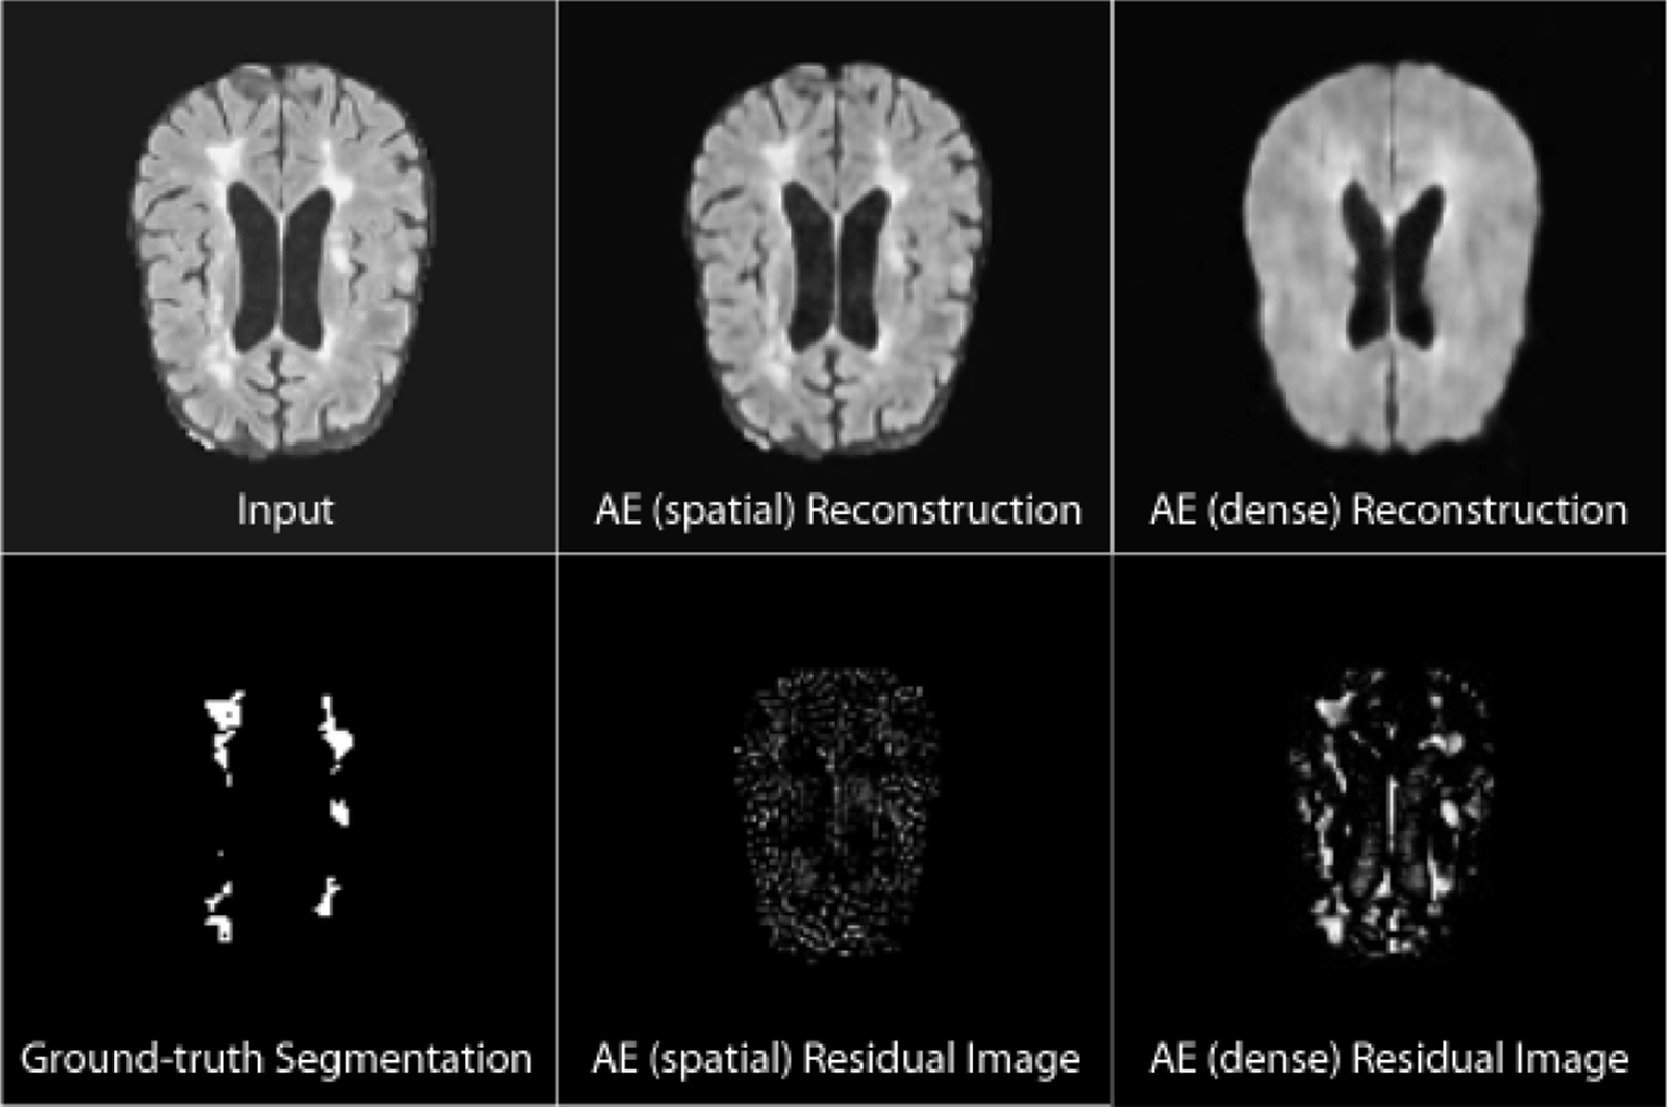
\includegraphics[width=0.7\textwidth]{figures/ae_failure.jpg}
    \caption{More performant autoencoders (middle column) will happily reconstruct anomalies with high accuracy, making them less appropriate for anomaly detection. However, less performant autoencoders (right column) will result in more false positives. How are practitioners supposed to determine the sweet spot? I argue that the autoencoding objective is inappropriate for anomaly detection from the start.}
    \label{fig:ae_failure}
\end{figure}%


\subsection*{The Curious Failure of Likelihood Models}

\begin{figure}[tbhp]
% \begin{subfigure}[t]{0.4\textwidth}
    \centering
    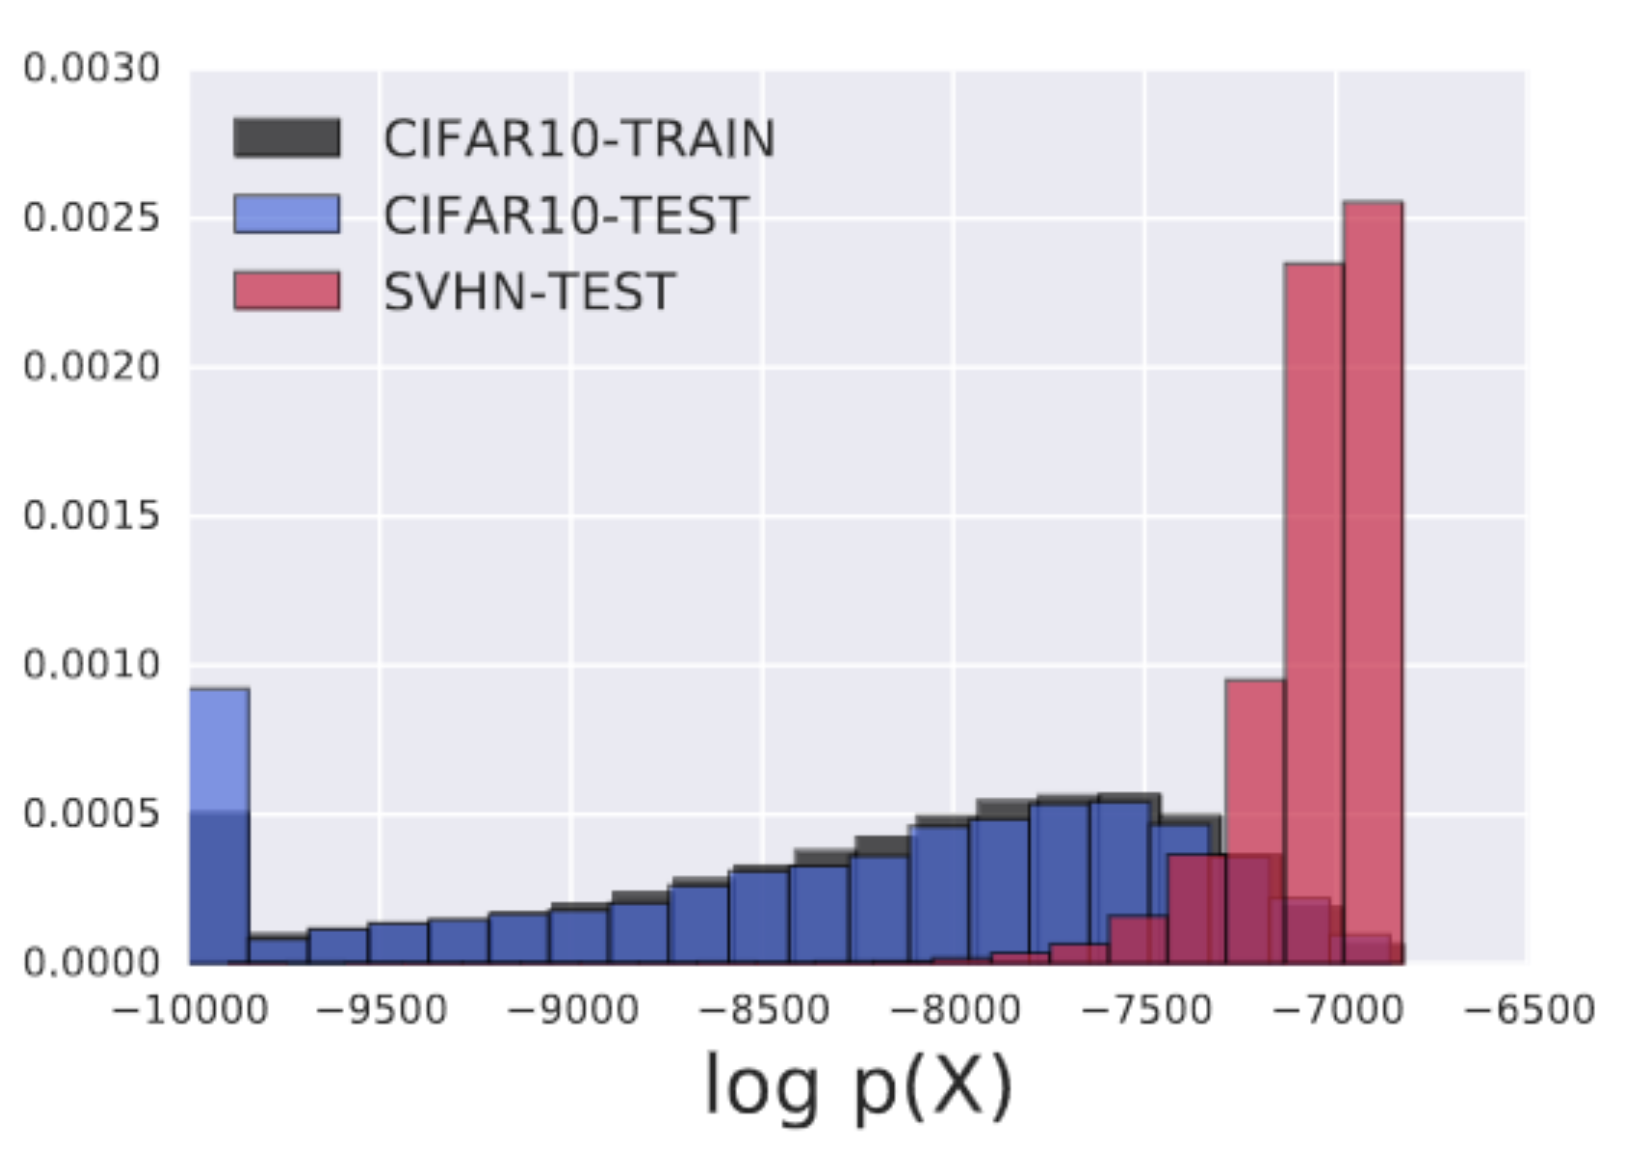
\includegraphics[width=.6\textwidth]{figures/cifar_glow_nalisnick.png}
    \caption{Log-likelihoods reported by a Glow model trained on CIFAR-10 (natural images). Note how it assigns \textit{higher} likelihoods to the out-of-distribution SVHN (street view housing number) images. This behavior is paradoxical and yet to be fully understood.}
    \label{fig:cifar_glow}
% \end{subfigure}
\end{figure}

Likelihood models are a natural candidate for anomaly detection. In fact, most definitions of the term `anomaly" invoke some flavor of probability. Further still, in the past decade, there have been many exciting advances in deep likelihood models such as PixelCNN, Glow, and an explosion of an entire class of so-called normalizing flow models.

These methods will estimate the probability densities of the samples with respect to a training distribution. A high probability density is an indication that the data point belongs to a set of samples that are likely to occur.
Conversely, out-of-distribution (OOD) samples will tend to reside in low-density probability regions.


So why not use deep likelihood models for anomaly detection? While these models often demonstrate exceptional generative capabilities, they frequently fail at detecting outlying samples. In fact, they often assign \textit{higher} likelihood to OOD samples. This curious failure of OOD detection has been extensively reported \cite{nalisnick2018do,why_norm_fails,nalisnick2020detecting} but has yet to be fully understood.

Some candidate explanations point to the overfitting of models to low-level features in the images. Of course, this argument only holds for vision models, whereas to my knowledge, the failure of deep likelihood models is agnostic to the data modality.

Another argument questions the typical set hypothesis.
The typical set of a probability distribution is the set whose elements have an information content sufficiently close to that of the expected information~\cite{shannon_1948}.
Researchers prescribing to this school-of-thought argue that high dimensional probability density functions may not correspond with our intuitions of probability. In high-dimensional Gaussians, the typical set resides in a thin shell at a specific distance from the center. Thus, a sample may belong to a typical set and yet need not lie in a high-density region. This is the so-called "Gaussian Soap Bubble" phenomenon and is rigorously proved in \cite{vershynin2018high}

%%%%%
% TODO:
%%%%z

\section{Score-Matching for Predicting Anomalies}

In this thesis, I will develop a case for a particular methodology, called denoising score matching, as a promising solution to unsupervised anomaly detection. By estimating the score (gradient of the log-probability-density), score matching estimates how far a given data point is from the data distribution. Conceptually, a score is a vector field that points in the direction where the likelihood increases the most. In the context of anomaly detection in medical imaging, score matching offers a powerful, yet under-explored, tool to discern pathological patterns from normal variations.

I posit that a multi-scale analysis of score estimates can effectively identify anomalies stemming from multiple underlying factors. In this research, I interpret "multi-scale" to imply multiple noise levels of perturbation. Intuitively, higher noise levels obscure local information, forcing the model to learn more global patterns. Therefore, by utilizing multiple noise levels during training, both global and local contextual features can be captured. This multi-scale capacity is particularly beneficial for anomaly detection in medical images, where anomalies may manifest as localized textures or as large-scale structures.


Note that the idea of using gradients of the log density as a means of outlier detection has been done in the past, most notably by \cite{Grathwohl2020Your, pmlr-v48-zhai16}. However, a bit surprisingly, neither work explicitly connected their ideas to score matching. \cite{Grathwohl2020Your} described the norm of the gradient of the log-density as "Approximate Mass", obtained from an Energy-Based Model (EBM). The authors even noted how the Approximate Mass predictor greatly outperformed likelihoods for the OOD task but did not explore the idea further. Their work can be considered as special-case of my proposed method: a single scale score estimator trained with sufficiently low noise would be estimating the gradient norms of the true log density. I will note that my technique significantly outperforms Approximate Mass, as reported in~\cite{mahmood2021multiscale}. \cite{pmlr-v48-zhai16} chanced upon gradient norms while exploring energy-based models for outlier detection. They correctly identified how reconstruction errors obtained via an energy-based model would correspond to the gradient of the log density. However, they did not see an improvement over simply using the energy scores. I posit that they too would have seen improvements by adopting a multi-scale approach. 

To my knowledge, my work has been the first to explore anomaly detection from the perspective of score matching. This thesis is also the first to empirically underscore the effectiveness of multiple noise scales for this task.


\section{Defining the term Anomaly}
As of yet, there is no standard definition of the term anomaly. 
For the purpose of my research, I will opt for a fairly loose definition of the term: any data point that does not belong to the typical set. That is, an anomaly is a sample with low probability \textit{mass}, with respect to the distribution described by the training data. 

Note that the diversity of my training samples will always be a limiting factor for the anomaly detection performance. It is very possible to encounter samples that human experts will categorize as typical but may seem out-of-distribution to a model trained on limited data. This is an inherent limitation of all learning technique, and one should be mindful of such limitations.

\section{Thesis Statement}

